\subsection{Gestion du code source}

\begin{frame}{Systèmes de gestion de versions}
\begin{itemize}[<+->]
 \item Local~:
 \begin{itemize}[<+->]
  \item SCCS~: remplacé par~:
  \item RCS~: remplacé par~:
 \end{itemize}
 \item Client-serveur~:
 \begin{itemize}[<+->]
  \item Tous ceux utilisés actuellement.
 \end{itemize}
 \item Deux modes principaux~:
 \begin{itemize}
 \item Centralisé
 \item Décentralisé
 \end{itemize}
\end{itemize}
\end{frame}

\begin{frame}{Systèmes de gestion de versions centralisés}
\begin{itemize}[<+->]
 \item Principe~:
 \begin{itemize}
  \item Chaque modification (commit) est envoyée directement sur le serveur.
 \end{itemize}
 \item Les plus connus~:
 \begin{itemize}[<+->]
  \item CVS
  \item Subversion
 \end{itemize}
 \item Inconvénient~: Nécessite une connexion pour envoyer ses modifications.
\end{itemize}
\end{frame}

\begin{frame}{Systèmes de gestion de versions décentralisés}
\begin{itemize}[<+->]
 \item Principe~:
 \begin{itemize}
  \item Chaque modification (commit) est stockée localement.
  \item L'ensemble des modifications est envoyée à un dépôt distant (remote)~;
  \item Possibilité d'avoir plusieurs dépôts distants.
 \end{itemize}
 \item Les plus connus~:
 \begin{itemize}[<+->]
  \item BitKeeper
  \item Git
  \item Mercurial
  \item GNU Bazaar (successeur de GNU Arch)
 \end{itemize}
 \item Avantage~: Pas besoin de connexion pour commiter~;
 \item Inconvénient~: Workflow plus complexe.
\end{itemize}
\end{frame}

\begin{frame}{Lexique}
\begin{description}[align=left]
 \item [Trunk] version de développement principale~;
 \begin{itemize}[<+->]
  \item Très instable~;
  \item Version à partir de laquelle on crée les branches et les tags~;
  \item Appelé aussi 'master' (Git).
 \end{itemize}
 \pause
 \item [Tags] version figée (release)~;
 \begin{itemize}[<+->]
  \item Ne doit pas être modifié directement\dots
  \item \dots donc utilisation de branches de maintenance.
 \end{itemize}
 \pause
 \item [Branche] version de développement secondaire~;
 \begin{itemize}[<+->]
  \item Branche de maintenance de version (hotfix)~;
  \item Branche de fonctionnalité (feature).
 \end{itemize}
 \pause
 \item [Révision/commit] modification atomique d'un ou plusieurs fichiers~;
 \pause
 \item [Head] dernière révision du dépôt~;
 \pause
 \item [Objet] élément versionnable (fichier, répertoire, lien symbolique, etc.).
\end{description}
\end{frame}

\begin{frame}{Utilisation générale}
\framesubtitle{Que faut-il versionner~?}
\begin{itemize}[<+->]
 \item Tout ce qui est susceptible d'être modifié au cours du temps~:
 \begin{itemize}[<+->]
  \item Code source~;
  \item Script de construction~;
  \item Documentation.
 \end{itemize}
 \item Mais pas ce qui est générable~:
 \begin{itemize}[<+->]
  \item Code compilé~;
  \item Documentation d'API~;
  \item Etc.~;
  \item Les différents systèmes possèdent un mécanisme d'ignore.
 \end{itemize}
\end{itemize}
\end{frame}

\begin{frame}{Utilisation générale}
\framesubtitle{Quand faut-il commiter~?}
\begin{itemize}[<+->]
 \item Le plus souvent possible~;
 \item Quand ça marche~:
 \begin{itemize}[<+->]
  \item Compile sans erreur~;
  \item Testé et validé.
 \end{itemize}
 \item Un commit inclut une modification et une seule.
 \begin{itemize}[<+->]
  \item Éviter les commits monolythiques.
 \end{itemize}
\end{itemize}
\end{frame}

\begin{frame}[fragile]{Subversion}
\framesubtitle{Informations générales}
\begin{itemize}[<+->]
 \item Anciens développeurs de CVS~;
 \item Première version en 2000\dots
 \item \dots version 1.0.0 en 2004~;
 \item Dernière version~:1.9.5 (29 novembre 2016)~;
 \item Un dépôt central, sur un serveur, sur les protocoles~:
 \begin{itemize}[<+->]
  \item SVN (svnserve, TCP 3690)~;
  \item HTTP (webdav, passe dans plus d'infrastructures réseau).
 \end{itemize}
 \item Pas de notion de branche ou de tag, utilisation de l'arborescence~;
 \item Possibilité de checkout une sous-arborescence~;
 \item Numéros de versions séquentiels, globaux au dépôt~;
 \item Les répertoires sont versionnés (notamment les répertoires vides)~;
 \item \url{http://svnbook.red-bean.com/} (assez ancienne, mais toujours d'actualité).
\end{itemize}
\end{frame}

\begin{frame}{Subversion}
\framesubtitle{Architecture d'un dépôt}
  \begin{itemize}[<+->]
   \item trunk
   \begin{itemize}[<+->]
    \item Développements courants~;
   \end{itemize}
   \item branches
   \begin{itemize}[<+->]
    \item Développements conséquents~;
    \item Maintenances de versions~;
   \end{itemize}
   \item tags
   \begin{itemize}[<+->]
    \item Versions figées~;
    \item Pas de modification dans les tags~;
   \end{itemize}
 \end{itemize}
\end{frame}

\begin{frame}{Subversion}
\framesubtitle{Architecture d'un dépôt}
 \begin{figure}
   \caption{Worflow de développement avec Subversion.}
   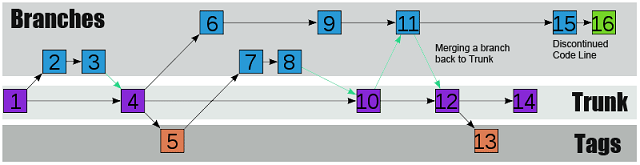
\includegraphics[width=345pt]{repository-structure3}\par
   \tiny Source~: \url{http://blogs.wandisco.com/2011/10/24/subversion-best-practices-repository-structure/}
 \end{figure}
\end{frame}

\begin{frame}{Subversion}
\framesubtitle{Workflow de développement}
\begin{description}
 \item [\Q{svn checkout}] créer sa copie locale~;
 \pause
 \item [\Q{svn update}] mettre à jour sa copie locale avec les modifications des autres~;
 \pause
 \item [\Q{svn add}] ajouter des fichiers~;
 \pause
 \item [\Q{svn copy}] copier des fichiers ou une sous-arborescence~;
 \begin{itemize}
  \item Sert particulièrement à créer les branches et les tags.
 \end{itemize}
 \pause
 \item [\Q{svn delete}] supprimer des fichiers~;
 \pause
 \item [\Q{svn move}] déplacer des fichies~;
 \pause
 \item [\Q{svn status}] voir l'état de la copie locale~;
 \pause
 \item [\Q{svn diff}] voir les différences entre deux versions, ou de sa copie locale par rapport à la dernière mise à jour du dépôt~;
 \pause
 \item [\Q{svn revert}] annuler une modification application inversée du diff d'un commit)~;
 \pause
 \item [\Q{svn resolve}] effectuer une gestion des conflits sur un fichier~;
 \pause
 \item [\Q{svn resolved}] marquer un conflit comme résolu~;
 \pause
 \item [\Q{svn commit}] pousser ses modifications sur le dépôt~;
 \pause
 \item [\Q{svn merge}] fusionner une branche dans une autre~;
 \pause
 \item [\Q{svn switch}] changer de branche (changer le point d'origine dans l'arborescence distante)~;
 \pause
 \item [\Q{svn info}] avoir les informations de sa copie locale.
\end{description}
\end{frame}

\begin{frame}[fragile]{Subversion}
\frametitle{svn status}
\begin{itemize}[<+->]
 \item Affiche l'état de la copie locale~;
 \item Permet d'avoir les modifications sur le serveur avec l'option \verb/--show-updates/ ou \verb/-u/~;
\end{itemize}
\begin{snvlisting}{Exemple d'invocation (honteusement copié sur \url{http://svnbook.red-bean.com/en/1.8/svn.ref.svn.c.status.html})}[][escapeinside={}]
# svn status -u wc
 M            965    wc/bar.c
        *     965    wc/foo.c
A  +          965    wc/qax.c
Status against revision:    981
\end{snvlisting}
\end{frame}

\begin{frame}[fragile]{Subversion}
\frametitle{svn status -- format}
\begin{itemize}[<+->]
 \item Première colonne~: changements sur l'objet~:
 \begin{description}[align=left]
  \item [\textvisiblespace] objet inchangé~;
  \item [A] objet ajouté (\verb/svn add/)~;
  \item [D] objet supprimé (\verb/svn delete/)~;
  \item [M] objet modifié~;
  \item [C] objet en conflit (après \verb/svn update/)~;
  \item [I] objet ignoré~;
  \item [?] objet inconnu (non ajouté)~;
  \item [!] objet manquant (supprimé du système de fichiers mais pas avec \verb/svn delete/)
  \item [\textasciitilde] objet ayant changé de type (par ex.~: fichier -> répertoire)
 \end{description}
\end{itemize}
\end{frame}

\begin{frame}[fragile]{Subversion}
\frametitle{svn status -- format}
\begin{itemize}[<+->]
 \item Seconde colonne~: changements sur les propriétés de l'objet~:
 \begin{description}[align=left]
  \item [\textvisiblespace] propriétés inchangées~;
  \item [M] propriétés modifiées~;
  \item [C] propriétés en conflit (modifiées localement et sur le dépôt distant).
 \end{description}
 \item Troisième colonne~: L si copie locale verrouillée~;
 \item Quatrième colonne~: + si ajout avec historique~;
 \item Cinquième colonne~: S si l'objet a changé de branche~;
 \item Sixième colonne~: informations de verrouillage distant~;
 \item Septième colonne~: informations de conflit d'arbre~;
 \item Huitième colonne~: toujours une espace~;
 \item Neuvième colonne~: * si l'objet est périmé (mis à jour sur le dépôt distant)~;
 \item Révision locale (si \verb/--show-updates/ ou \verb/--verbose/ passé en paramètre)~;
 \item Dernière révision commitée (si \verb/--verbose/ passé en paramètre)~;
 \item Toujours en dernier~: chemin de l'objet concerné, peut contenir des espaces.
\end{itemize}
\end{frame}

\begin{frame}[fragile]{Subversion}
\frametitle{svn info}
\begin{snvlisting}{Exemple d'invocation (honteusement copié sur \url{http://svnbook.red-bean.com/en/1.8/svn.ref.svn.c.info.html})}[][escapeinside={}]
# svn info foo.c
Path: foo.c
Name: foo.c
Working Copy Root Path: /home/sally/projects/test
URL: http://svn.red-bean.com/repos/test/foo.c
Repository Root: http://svn.red-bean.com/repos/test
Repository UUID: 5e7d134a-54fb-0310-bd04-b611643e5c25
Revision: 4417
Node Kind: file
Schedule: normal
Last Changed Author: sally
Last Changed Rev: 20
Last Changed Date: 2003-01-13 16:43:13 -0600 (Mon, 13 Jan 2003)
Text Last Updated: 2003-01-16 21:18:16 -0600 (Thu, 16 Jan 2003)
Properties Last Updated: 2003-01-13 21:50:19 -0600 (Mon, 13 Jan 2003)
Checksum: d6aeb60b0662ccceb6bce4bac344cb66
\end{snvlisting}
\end{frame}

\begin{frame}[fragile]{Subversion}
\frametitle{Propriétés}
\begin{itemize}[<+->]
 \item Métadonnées des objets~;
 \item Clé-valeur~;
 \item Personnalisées ou réservées à subversion (préfixées par \verb/svn:/)
 \item Commandes~:
 \begin{description}
  \item [\Q{svn proplist <objet>}] affiche les propriétés d'un objet~;
  \item [\Q{svn propedit <nom> <objet>}] ouvre un éditeur pour définir la valeur d'une propriété d'un objet~;
  \item [\Q{svn propset <nom> <valeur> <objet>}] définit la valeur d'une propriété d'un objet~;
  \item [\Q{svn propdel <nom> <objet>}] supprime la propriété de l'objet.
 \end{description}
 \item Quelques propriétés connues~:
 \begin{description}
  \item [\Q{svn:ignore}] liste des objets non versionnés~;
  \item [\Q{svn:eol-style}] type de fin de ligne (unix, dos)~;
  \item [\Q{svn:author}] auteur de la révision~;
  \item [\Q{svn:date}] date de la révision~;
  \item [\Q{svn:log}] message de révision.
 \end{description}
\end{itemize}
\end{frame}

\begin{frame}[fragile]{Subversion}
\frametitle{\Q{svn:ignore}}
\begin{itemize}[<+->]
 \item Contient la liste des patterns d'objets ignorés~;
 \item S'applique à un répertoire.
\end{itemize}
\begin{snvlisting}{Exemple}[][escapeinside={}]
*~
.*.sw*
*.pyc
\end{snvlisting}
\end{frame}

\begin{frame}{Subversion}
 \framesubtitle{Outils annexes}
 \begin{description}
  \item [TortoiseSVN] Intégration dans l'explorateur de fichiers Windows~;
  \pause
  \item [eSVN] Interface graphique dédiée, multiplateforme~;
  \pause
  \item [kdesvn] Interface graphique dédiée, Linux uniquement~;
  \pause
  \item [Différents IDE] La plupart des IDE ont une intégration de subversion~;
  \pause
  \item [Forges] Outils web intégrés pour le développement.
  \pause
  \item [Etc.] Modules d'éditeurs de texte, intégration gestionnaires de fichiers, \dots
  \pause
 \end{description}
\end{frame}

\begin{frame}[fragile]{Git}
\frametitle{Informations générales}
\begin{itemize}[<+->]
 \item Initialement écrit par Linus Torvalds pour remplacer BitKeeper~;
 \item Première version le 7 avril 2005~;
 \item Dernière version le 4 août 2017 (2.14.1)~;
 \item Possibilité d'avoir plusieurs dépôts distants (remote)~;
 \item Accessibles via les protocoles~:
 \begin{itemize}
  \item SSH (authentification par clé)
  \item HTTP (clonage anonyme)
  \item git (en pratique peu utilisé)
 \end{itemize}
 \item La copie locale est un clone (complet ou incomplet) du dépôt distant~;
 \item Notions de tags et de branches~;
 \item Pas de séquence, utilisation de hash pour identifier les commits~;
 \item Les répertoires ne sont pas versionnés, donc absence de répertoires vides~;
 \item Possibilité d'étendre la commande (\verb/git flow/ par exemple)~;
 \item \url{https://git-scm.com/book/fr/v2/}.
\end{itemize}
\end{frame}

\begin{frame}{Git}
\framesubtitle{Terminologie}
\begin{description}
 \item [blob] contenu d'un objet versionné (fichier)~;
 \pause
 \item [commit] révision, hash et commit parent~;
 \pause
 \item [branche] version active du projet~;
 \pause
 \item [tag] étiquette sur un point donné de l'historique, permet de figer des releases~;
 \pause
 \item [merge] fusion entre deux branches~;
 \pause
 \item [rebase] changement de la base de la branche par une autre branche~;
 \pause
 \item [staging] aussi appelé cache, contient les objets et états servant au commit~;
 \pause
 \item [stash] pile dans laquelle le développeur peut stocker ses modifications sans les commiter, souvent avant un pull pour fusionner ses modifications a posteriori.
\end{description}
\end{frame}

\begin{frame}{Git}
\framesubtitle{Workflow}
\begin{description}
 \item [\Q{git clone}] clone un dépôt distant en local~;
 \pause
 \item [édition] modifie les fichiers~;
 \pause
 \item [\Q{git stash}] sauvegarde les modifications dans stash~;
 \pause
 \item [\Q{git pull}] récupére les révisions distantes~;
 \pause
 \item [\Q{git stash pop}] réapplique les modifications sur la copie de travail à jour~;
 \pause
 \item [\Q{git mergetool}] lance l'outil de gestion des conflits (lors d'un pull, ou d'un merge)~;
 \pause
 \item [\Q{git add}] ajoute un fichier modifié ou non versionné dans le cache~;
 \pause
 \item [\Q{git rm}] supprime un fichier et le met comme tel dans le cache~;
 \pause
 \item [\Q{git commit}] crée une révision locale d'après le cache~;
 \pause
 \item [\Q{git push}] pousse les révisions locales~;
\end{description}
\end{frame}
 
\begin{frame}{Git}
\framesubtitle{Workflow -- suite}
\begin{description}
 \item [\Q{git branch}] manipule les branches~;
 \pause
 \item [\Q{git checkout}] change de branche, ou restaure un fichier de travail~;
 \pause
 \item [\Q{git reset}] réinitialise HEAD à un état différent~;
 \pause
 \item [\Q{git merge}] fusionne une branche dans la branche courante~;
 \pause
 \item [\Q{git mergetool}] lance l'outil de gestion des conflits si nécessaire~;
 \pause
 \item [\Q{git rebase}] reconstruit l'historique de la branche par rapport à une autre branche~;
 \pause
 \item [\Q{git tag}] manipule les tags, possibilité de le signe avec une clé PGP.
\end{description}
\end{frame}

\begin{frame}[fragile]{Git}
\frametitle{Autres commandes utiles}
\begin{description}
 \pause
 \item [\Q{git blame}] affiche le commit et l'auteur de chaque ligne d'un fichier~;
 \pause
 \item [\Q{git diff}] affiche les différences sur la copie locale, ou entre deux révisions~;
 \begin{itemize}[<+->]
  \item Permet de générer un fichier patch, avec l'option \verb/--patch/ ou \verb/-p/ ou encore \verb/-u/~;
 \end{itemize}
 \pause
 \item [\Q{git submodule}] gère les sous-modules~;
 \pause
 \item [\Q{git help <command>}] RTFM ;-) Attention, très (trop) complet.
\end{description}
\end{frame}

\begin{frame}{Git}
 \frametitle{Workflow simple}
 \begin{figure}
   \caption{Worflow de développement local avec Git.}
   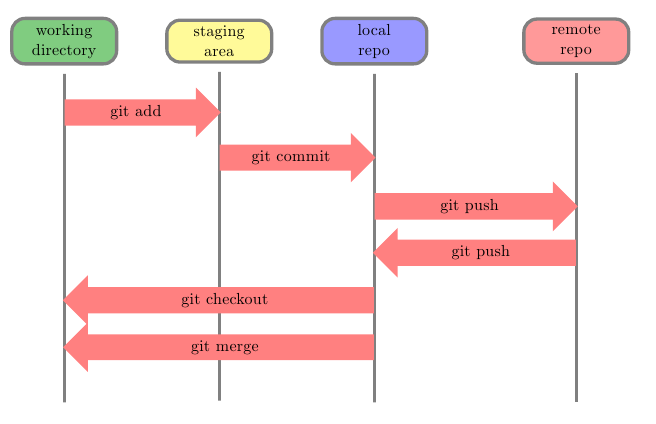
\includegraphics[height=160pt]{git-base-workflow}\par
   \tiny Source~: \url{http://tex.stackexchange.com/questions/70320/workflow-diagram}
 \end{figure}
\end{frame}

\begin{frame}[fragile]{Git}
\frametitle{\Q{git status}}
\begin{snvlisting}{Exemple}[][escapeinside=||]
On branch master
Your branch is up-to-date with 'origin/master'.
Changes to be committed:
  (use "git reset HEAD <file>..." to unstage)

        modified:   mailcap

Changes not staged for commit:
  (use "git add <file>..." to update what will be committed)
  (use "git checkout -- <file>..." to discard changes in working directory)

        modified:   caffrc
        modified:   config/i3pystatus/config.py
        modified:   dotfilesrc
        modified:   mutt-profiles/alexis@lahouze.org/profile
        modified:   mutt-profiles/alexis@sysnove.fr/profile
        modified:   offlineimaprc
        modified:   services/dunst/log/run
        modified:   tmux.conf
        modified:   vimrc
        modified:   zshrc

Untracked files:
  (use "git add <file>..." to include in what will be committed)

        config/flexget/
        imapnotify.js

\end{snvlisting}
\end{frame}

\begin{frame}[fragile]{Git}
\frametitle{Sous-modules}
\begin{itemize}[<+->]
 \item Référence de dépôts git dans des sous-répertoires du dépôt~;
 \item Ne se mettent pas à jour automatiquement~;
 \item Enregistré dans \verb/.gitmodules/~;
 \item Workflow~:
 \begin{itemize}[<+->]
  \item \verb/git submodule add/
  \item \verb/git commit -m "..."/
  \item \verb/git submodule update/
 \end{itemize}
 \item \url{https://git-scm.com/book/fr/v1/Utilitaires-Git-Sous-modules}
\end{itemize}
\end{frame}

\begin{frame}[fragile]{Git}
 \frametitle{Git Flow}
 \begin{itemize}[<+->]
  \item Décrit par Vincent Driesse sur \url{http://nvie.com/posts/a-successful-git-branching-model/}
  \item Process de développement et de publication standardisé~;
  \item Commande \verb/git flow/ (\url{https://github.com/nvie/gitflow}).
  \item Antisèche~: \url{http://danielkummer.github.io/git-flow-cheatsheet/}
 \end{itemize}
\end{frame}

\begin{frame}[fragile]{Git}
 \frametitle{Git Flow}
 \begin{figure}
   \caption{Workflow complet avec git flow.}
   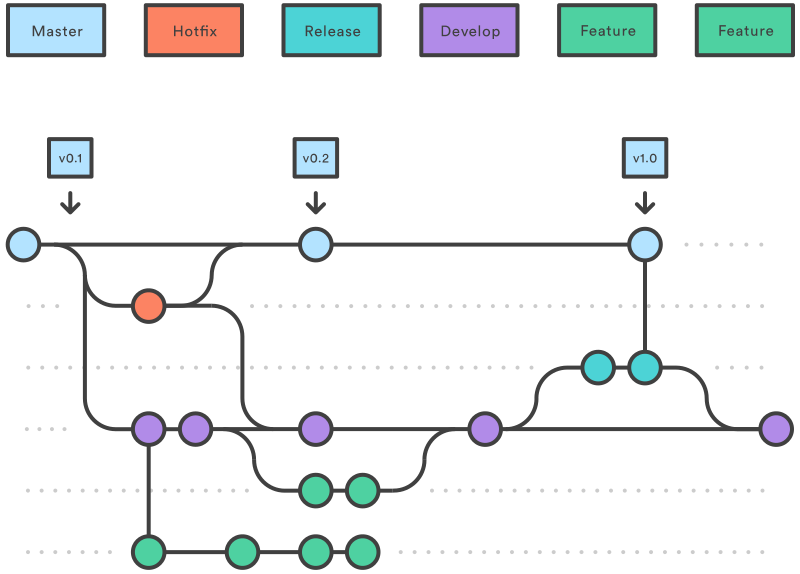
\includegraphics[height=160pt]{Gitflow-workflow}\par
   \tiny Source~: \url{https://www.atlassian.com/git/tutorials/comparing-workflows/gitflow-workflow}
 \end{figure}
\end{frame}

\begin{frame}[fragile]{Git}
\frametitle{git svn}
\begin{itemize}[<+->]
 \item Possibilité pour Git de se connecter à un dépôt Subversion~;
 \item Permet d'effectuer des commits locaux~;
 \item Ne permet pas de décentraliser le développement.
 \item \url{https://git-scm.com/book/fr/v2/Git-et-les-autres-systèmes-Git-comme-client#Git-et-Subversion}
\end{itemize}
\end{frame}

\begin{frame}[fragile]{Git}
\frametitle{git svn -- utilisation de base}
\begin{description}
 \item [\Q{git svn clone}] équivalent à \verb/svn checkout/~;
 \pause
 \item [\Q{git add}, \Q{git commit}] travailler localement~;
 \pause
 \item [\Q{git svn rebase}] équivalent à \verb/svn update/~;
 \pause
 \item [\Q{git svn dcommit}] équivalent à \verb/svn commit/ pour chaque commit local~;
 \pause
 \item [\Q{git svn branch}] manipule les branches et les tags (\verb/--tag/ ou \verb/--t/)~;
 \pause
 \item [\Q{git svn log}] affiche l'historique~;
 \pause
 \item [\Q{git svn blame}] affiche l'auteur et la révision de chaque ligne d'un fichier~;
 \pause
 \item [\Q{git svn reset}] permet de revenir à une révision spécifique~;
 \pause
 \item [\Q{git svn help}] RTFM ;-)
\end{description}
\end{frame}

\begin{frame}[fragile]{Git}
 \frametitle{Exemples - Cas simple}
 \begin{itemize}[<+->]
  \item Créer un dépôt sur Github
  \item Configurer son git local (user, email)
  \item Initialiser la copie locale
  \item Ignorer les fichiers constructibles, temporaires, etc.
  \item Ajouter les fichiers nécessaires au projet
  \item Commiter la branche \verb/master/
  \item Créer une branche \verb/develop/ et basculer dessus
  \item Ajouter un fichier README
  \item Ajouter dans le cache
  \item Commiter
  \item Modifier un fichier
  \item Ajouter dans le cache
  \item Commiter
  \item Merger dans \verb/master/
 \end{itemize}

\end{frame}
